\documentclass[10pt,a4paper]{article}

\usepackage{amsmath}
\usepackage{amsthm}
\usepackage{multicol}
\usepackage{color}
\usepackage{verbatim}
\usepackage{semantic}
\usepackage{wasysym}
\usepackage{charter}
\usepackage{stmaryrd}
\usepackage{graphicx}

\newtheorem{definition}{Definition}

\newcommand{\kvd}[1]{\textbf{#1}}
\newcommand{\ident}[1]{\textit{#1}}
\newcommand{\val}[1]{\texttt{#1}}
\newcommand{\calv}{\mathcal{V}}
\newcommand{\calr}{\mathcal{R}}

\begin{document}

\title{Type providers}
\author{Tomas Petricek} 
\maketitle

% ==================================================================================================

\section{Introduction}
TBD
\begin{itemize}
\item \textbf{Information spaces} describes what?
\item \textbf{Schema} describes what?
\end{itemize}

\newpage
\section{Formal model}

\subsection{Information spaces}
The first problem in formalizing type providers is to find a formal model of \emph{information space}
that is simple and amenable to formal analysis, but powerful enough to model a wide range of data
sources accessible using type providers including hierarchical data (i.e.\ XML files), SQL databases, 
multi-dimensional data (such as the World Bank data set) etc. 

We model information spaces simply as undirected graph with values as vertices and relations
between values as edges.

\begin{definition}
An \emph{information space} $(\calv, \calr)$ is a tuple of values $\calv$ and relations between
pairs of values $\calr \in \calv \times \calv$. The relations are undirected, meaning that 
$(v_1, v_2) \in \calr \Leftrightarrow (v_2, v_1) \in \calr$. 
\end{definition}

\subsection{Examples} 
To demonstrate that the simple definition is general enough, we look at two examples 
that demonstrate how databases and XML data can be viewed as information spaces.

\paragraph{Databases.} For simplicity, we only consider database with a simple table 
(Products) with two columns (Name and Price) where the first column is the primary key.
The mapping is demonstrated in Figure~\ref{fig:infospace-db}.

The set of values is represented as dots in the figure. It is obtained by taking all 
data and meta-data information about the database. Assuming that $P$ is a collection of
table data indexed by $I$ (in our example, pairs consisting of name and price), we 
construct the set of values by taking name of the table, names of columns and all values:

\[
\calv = \{ \val{"Products"}, \val{"Name"}, \val{"Price"} \} \cup \bigcup_{i\in I}  \{n_i | (n_1, \ldots, n_k) \in P \}
\]

\begin{figure}
\begin{center}
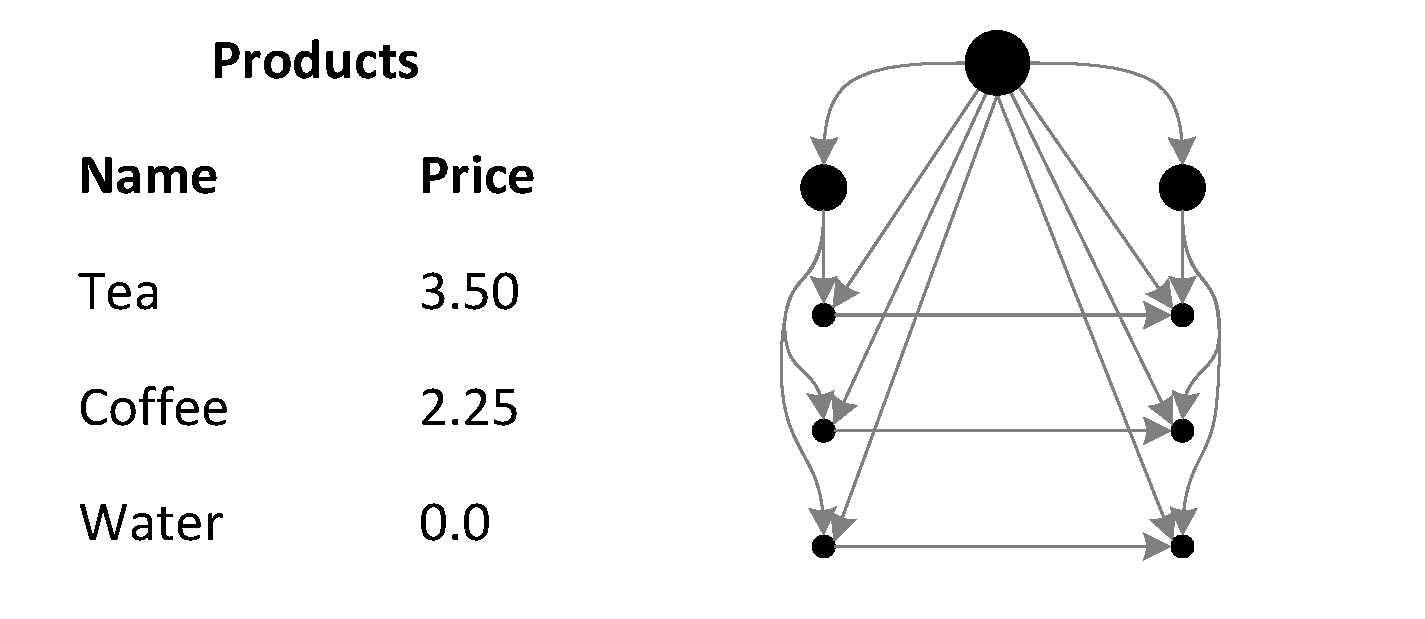
\includegraphics[scale=0.4]{figs/database.pdf}
\end{center}
\vspace{-1.5em}
\caption{Mapping database table to an information space}
\label{fig:infospace-db}
\end{figure}

\begin{figure}
\begin{center}
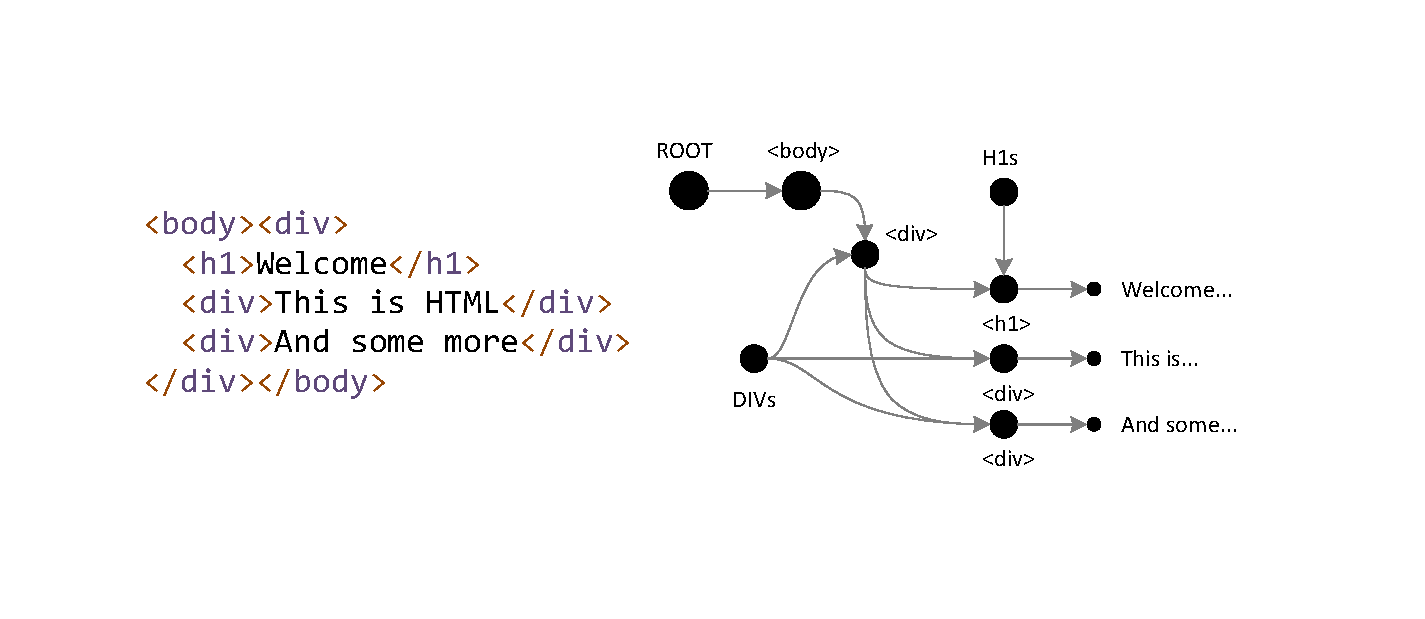
\includegraphics[scale=0.4]{figs/xml.pdf}
\end{center}
\vspace{-1.5em}
\caption{Stuff}
\label{fig:stuff2}
\end{figure}

\end{document}






























